\documentclass[a4paper,12pt]{article}
\usepackage[a4paper, margin=2.5cm]{geometry}
\usepackage[pdftex]{graphicx}
\usepackage{tikz}
\usepackage{float}
\usepackage[document]{ragged2e}
\usepackage[utf8]{inputenc}
\usepackage[T1]{fontenc}
\usepackage[spanish,es-tabla]{babel}
\renewcommand{\shorthandsspanish}{}
\usepackage{xurl}
\usepackage{lipsum}
\usepackage{mwe}
\usepackage{multicol}
\usepackage{siunitx}
\usepackage{listings}
\usepackage{circuitikz}

\graphicspath{ {/home/saikkopat/Documents/school/CE/"Tarea 2"/figures/} }

\title{Tarea 2: Reglas del divisor de voltaje y divisor de corriente}
\author{González Cárdenas Ángel Aquilez}

\begin{document}

\begin{titlepage}
	\begin{tikzpicture}[overlay, remember picture]
		\path (current page.north east) ++(-0.3,-1.5) node[below left] {
\includegraphics[width=0.35\textwidth]{/home/saikkopat/Documents/LOGOS IPN/EscudoESCOM}};
	\end{tikzpicture}
	\begin{tikzpicture}[overlay, remember picture]
		\path (current page.north west) ++(1.5,-1) node[below right] {
\includegraphics[width=0.2\textwidth]{/home/saikkopat/Documents/LOGOS IPN/logo}};
	\end{tikzpicture}
	\begin{center}
		\vspace{-1.5cm}
		{\LARGE Instituto Politécnico Nacional\par}
		\vspace{.5cm}
		{\LARGE Escuela Superior de Cómputo\par}
		\vspace{2.5cm}
		{\large Unidad de aprendizaje:}\\{\Large Circuitos Eléctricos\par}
		\vspace{2cm}
		{\scshape\Huge Tarea 2\par}
		{\itshape\Large Reglas del divisor de voltaje y divisor de corriente\par}
		\vfill
		\vspace{.7cm}
		{\Large Grupo: 3CV2\par}
		\vspace{.7cm}
		{\Large Alumno:\\González Cárdenas Ángel Aquilez\par}
		\vspace{1cm}
		{\Large Profesor: Vázquez Ortíz Mijaíl\par}
		\vspace{1cm}
		{\large Fecha de entrega: 21 de marzo de 2023\par}
		\vfill
	\end{center}
\end{titlepage} 

\newpage


\section*{Regla del divisor de corriente (RDC)}

\textbf{1.} Aplique la regla del divisor de corriente y encuentre las cantidades desconocidas usando la información proporcionada en el siguiente circuito:\par

\vspace{.5cm}

\begin{figure}[h!]
	\centering
	  \begin{circuitikz}[american, voltage dir=RP] 
	  		\draw	(0,0) 
	  		to[short, i=$\SI{6}{\uA}$] (2,0)
	  		to[R, l=$R$, i=$I_1$] (5,0)
			to[short, i=$I_3$] (7,0);
			\draw (2,0) -- (2,2)
			to[R, l=\SI{9}{\ohm}, i=$\SI{2}{\uA}$] (5,2) -- (5, 0);
			\draw (2,0) -- (2,-2)
			to[R, l=\SI{9}{\ohm}, i=$I_2$] (5,-2) -- (5,0);
		\end{circuitikz}
	\caption{Circuito en paralelo}
\end{figure}

\vspace{.5cm}

Partiendo de la definición de la regla del divisor de corriente, sabemos que:

\[
	iR_x = \frac{i_t \times R_t}{R_x}
\]

donde podemos despejar $R_t$, así

\[
	R_t = \frac{iR_x \times R_x}{i_t}
\]

y para el primer resistor de \SI{9}{\ohm} que tiene una corriente de \SI{2}{\uA},

\[
	R_t = \frac{\SI{2}{\uA} \times \SI{9}{\ohm}}{\SI{6}{\uA}} = \SI{3}{\ohm}
\]

luego, con la regla del divisor de corriente, para el ultimo resistor se tiene que

\[
	i_2 = \frac{\SI{6}{\uA} \times \SI{9}{\ohm}}{\SI{9}{\ohm}} = \SI{2}{\uA}
\]

Ahora, para encontrar el valor de la corriente $i_1$ que pasa a través del resistor $R$, supongamos que la corriente se divide de forma equitativa entre los tres resistores en paralelo, lo que implica que:

\[
	\SI{6}{\uA} = \SI{2}{\uA} + i_1 + i_2 = \SI{2}{\uA} + \SI{2}{\uA} + i_1
\]

de donde

\[
	i_1 = \SI{6}{\uA} - \SI{2}{\uA} - \SI{2}{\uA} = \SI{2}{\uA}
\]
luego, despejando $R_x$ de la regla del divisor de corriente, tenemos que para R

\[
	R = \frac{\SI{6}{\uA} \times \SI{3}{\ohm}}{\SI{2}{\uA}} = \SI{9}{\ohm}
\]

que se comprueba con el valor de $R_t$, así

\[
	R_t = \frac{1}{\frac{1}{9} + \frac{1}{9} + \frac{1}{9}} \si{\ohm} = \SI{3}{\ohm}
\]

Por lo tanto, se concluye que la corriente se distribuye de manera equitativa por lo que

\[
	i_3 = \SI{6}{\uA}
\]

\section*{Regla del divisor de voltaje (RDV)}

\textbf{2.} Aplicando la regla del divisor de voltaje, determine el voltaje $V_0$ para el siguiente circuito:\par

\vspace{.5cm}

\begin{figure}[h!]
	\centering
	  \begin{circuitikz}[american, voltage dir=RP] 
	  		\draw	(0,0) 
			to[vsource,l=\SI{12}{\volt}] (0, 3)
			to[R, l=\SI{20}{\ohm}] (3,3)
			to[R, l=\SI{8}{\ohm}] (6,3)
			to[R, l=\SI{10}{\ohm}] (9,3) -- (9.7, 3)
			to[R, l=\SI{20}{\ohm}, v=$V_0$] (9.7,0) -- (9,0)
			to[R, l=\SI{10}{\ohm}] (6,0)
			to[R, l=\SI{12}{\ohm}] (3,0) -- (0,0);
			\draw (3,3)
			to[R, a=\SI{40}{\ohm}] (3,0);
			\draw (6,3)
			to[R, a=\SI{40}{\ohm}] (6,0);
		\end{circuitikz}
	\caption{Circuito en serie-paralelo}
\end{figure}

\vspace{.5cm}

Para poder aplicar la regla del divisor de voltaje, se deberá de dibujar el circuito hasta su configuración equivalente mas simple, y empezando de derecha a izquierda, tenemos que

\[
Req_1 = \SI{10}{\ohm} + \SI{20}{\ohm} + \SI{10}{\ohm} = \SI{40}{\ohm}
\]
para el Circuito equivalente 1 en la Figura 3.

\begin{figure}[h!]
	\centering
	  \begin{circuitikz}[american, voltage dir=RP] 
	  		\draw	(0,0) 
			to[vsource,l=\SI{12}{\volt}] (0, 3)
			to[R, l=\SI{20}{\ohm}] (3,3)
			to[R, l=\SI{8}{\ohm}] (6,3) -- (8,3)
			to[R, l=$Req_1$, a=\SI{40}{\ohm}] (8,0) -- (6,0)
			to[R, l=\SI{12}{\ohm}] (3,0) -- (0,0);
			\draw (3,3)
			to[R, a=\SI{40}{\ohm}] (3,0);
			\draw (6,3)
			to[R, a=\SI{40}{\ohm}] (6,0);
		\end{circuitikz}
	\caption{Circuito equivalente 1}
\end{figure}

\vspace{.5cm}

De manera similar, para ambos resistores de 40\si{\ohm} de la derecha, tenemos que

\[
	Req_2 = \frac{40 \times 40}{80}\si{\ohm} = \SI{20}{\ohm}
\]

En la Figura 4 tenemos el circuito equivalente 2.

\begin{figure}[h!]
	\centering
	  \begin{circuitikz}[american, voltage dir=RP] 
	  		\draw	(0,0) 
			to[vsource,l=\SI{12}{\volt}] (0, 3)
			to[R, l=\SI{20}{\ohm}] (3,3)
			to[R, l=\SI{8}{\ohm}] (6,3)
			to[R, l=$Req_2$, a=\SI{20}{\ohm}] (6,0)
			to[R=12\si{\ohm}] (3,0) -- (0,0);
			\draw (3,3)
			to[R, a=\SI{40}{\ohm}] (3,0);
		\end{circuitikz}
	\caption{Circuito equivalente 2}
\end{figure}

\vspace{.5cm}

De manera similar, tenemos 

\[
Req_3 = \SI{8}{\ohm} + \SI{20}{\ohm} + \SI{12}{\ohm} = \SI{40}{\ohm}
\]

y el circuito equivalente 3 en la Figura 5.

\begin{figure}[h!]
	\centering
	  \begin{circuitikz}[american, voltage dir=RP] 
	  		\draw	(0,0) 
			to[vsource,l=\SI{12}{\volt}] (0, 3)
			to[R, l=\SI{20}{\ohm}] (3,3)
			to[R, a=\SI{40}{\ohm}] (3,0) -- (0,0);
			\draw (3,3) -- (5,3)
			to[R, a=\SI{40}{\ohm}, l=$Req_3$] (5,0) -- (3,0);
		\end{circuitikz}
	\caption{Circuito equivalente 3}
\end{figure}

\vspace{.5cm}

Luego, tenemos así

\[
	Req_4 = \frac{40 \times 40}{80}\si{\ohm} = \SI{20}{\ohm}
\]

Y finalmente, tenemos el circuito equivalente en su configuración mas simple en la Figura 6.

\begin{figure}[h!]
	\centering
	  \begin{circuitikz}[american, voltage dir=RP] 
	  		\draw	(0,0) 
			to[vsource,l=\SI{12}{\volt}] (0, 3)
			to[R, l=\SI{20}{\ohm}] (3,3)
			to[R, a=\SI{20}{\ohm}, l=$Req_4$] (3,0) -- (0,0);
		\end{circuitikz}
	\caption{Circuito equivalente 4: configuración mas simple}
\end{figure}

\vspace{.5cm}

Con la configuración mas simple del circuito, con sus resistores equivalentes en serie, partimos de la definición de la regla del divisor de voltaje:

\[
	V_x = \frac{E \times R_x}{R_t}
\]

Para el circuito equivalente 4, tenemos que $E = \SI{12}{\volt}, R_x = \SI{20}{\ohm}$, y  $R_t = \SI{40}{\ohm}$, entonces

\[
	V\textsubscript{{\SI{20}{\ohm}}} = \frac{\SI{12}{\volt} \times \SI{20}{\ohm}}{\SI{40}{\ohm}} = \SI{6}{\volt}
\]

y como $Req_4 = \SI{20}{\ohm}$, el voltaje es el mismo. Como el circuito equivalente 3 tiene dos resistores en paralelo, tenemos que $VReq_3 = VReq_4 = \SI{6}{\volt}$, y de forma similar tenemos $E = \SI{6}{\volt}, R_x = \SI{20}{\ohm}$, y  $R_t = \SI{40}{\ohm}$, entonces

\[
	V\textsubscript{{\SI{20}{\ohm}}} = \frac{\SI{6}{\volt} \times \SI{20}{\ohm}}{\SI{40}{\ohm}} = \SI{3}{\volt}
\]

De manera análoga, por su configuración en paralelo, tenemos que $VReq_2 = VReq_1 = \SI{3}{\volt}$, por lo que aplicando una vez mas la regla del divisor de voltaje con $E = \SI{3}{\volt}, R_t = \SI{40}{\ohm}$, para determinar el voltaje $V_0$, tenemos

\[
	V_0 = \frac{\SI{3}{\volt} \times \SI{20}{\ohm}}{\SI{40}{\ohm}} = \SI{1.5}{\volt}
\]

\newpage


\section*{Simulaciones}

Las siguientes simulaciones se realizaron utilizando el simulador mutiplataforma EveryCircuit\texttrademark.\par

\vspace{.5cm}

Para el primer circuito (Figura 1), la simulación de la Figura 7 comprueba los resultados del análisis utilizando la regla del divisor de corriente.

\vspace{.5cm}

\begin{figure}[!h]
\centering
	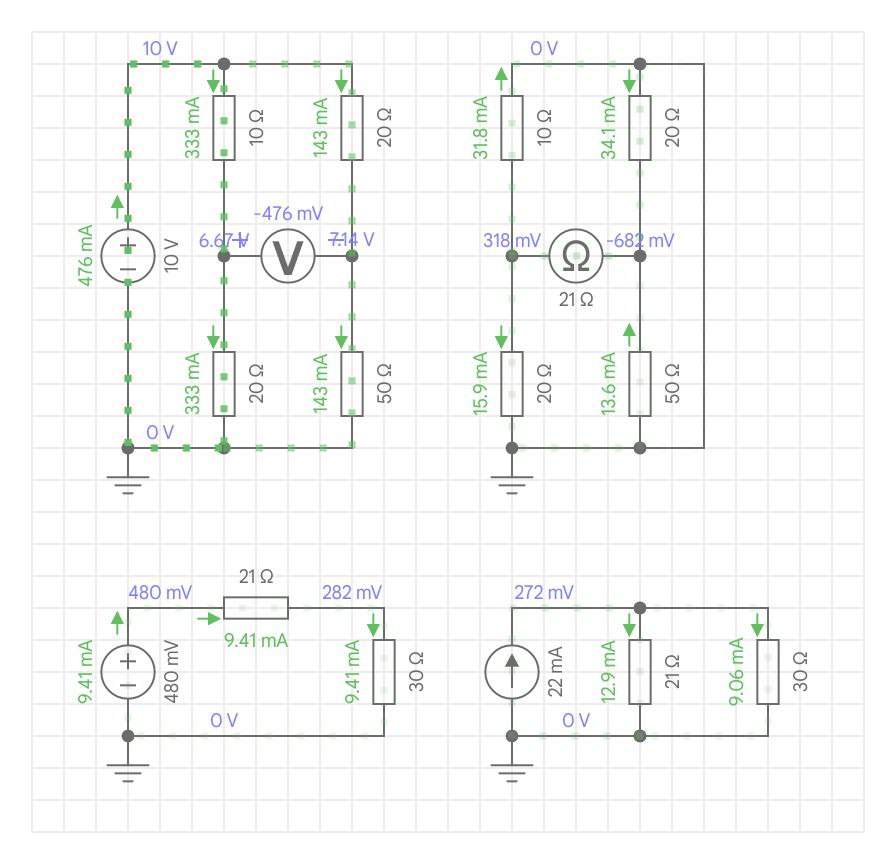
\includegraphics[width=.5\textwidth]{fig1}
	\label{fig5}
	 \caption{Simulación del circuito en paralelo de la Figura 1}
\end{figure}

\vspace{.5cm}

Y para el segundo circuito (Figura 2), la simulación de la Figura 8 comprueba el análisis hecho utilizando la regla del divisor de voltaje.

\vspace{.5cm}

\begin{figure}[!h]
\centering
	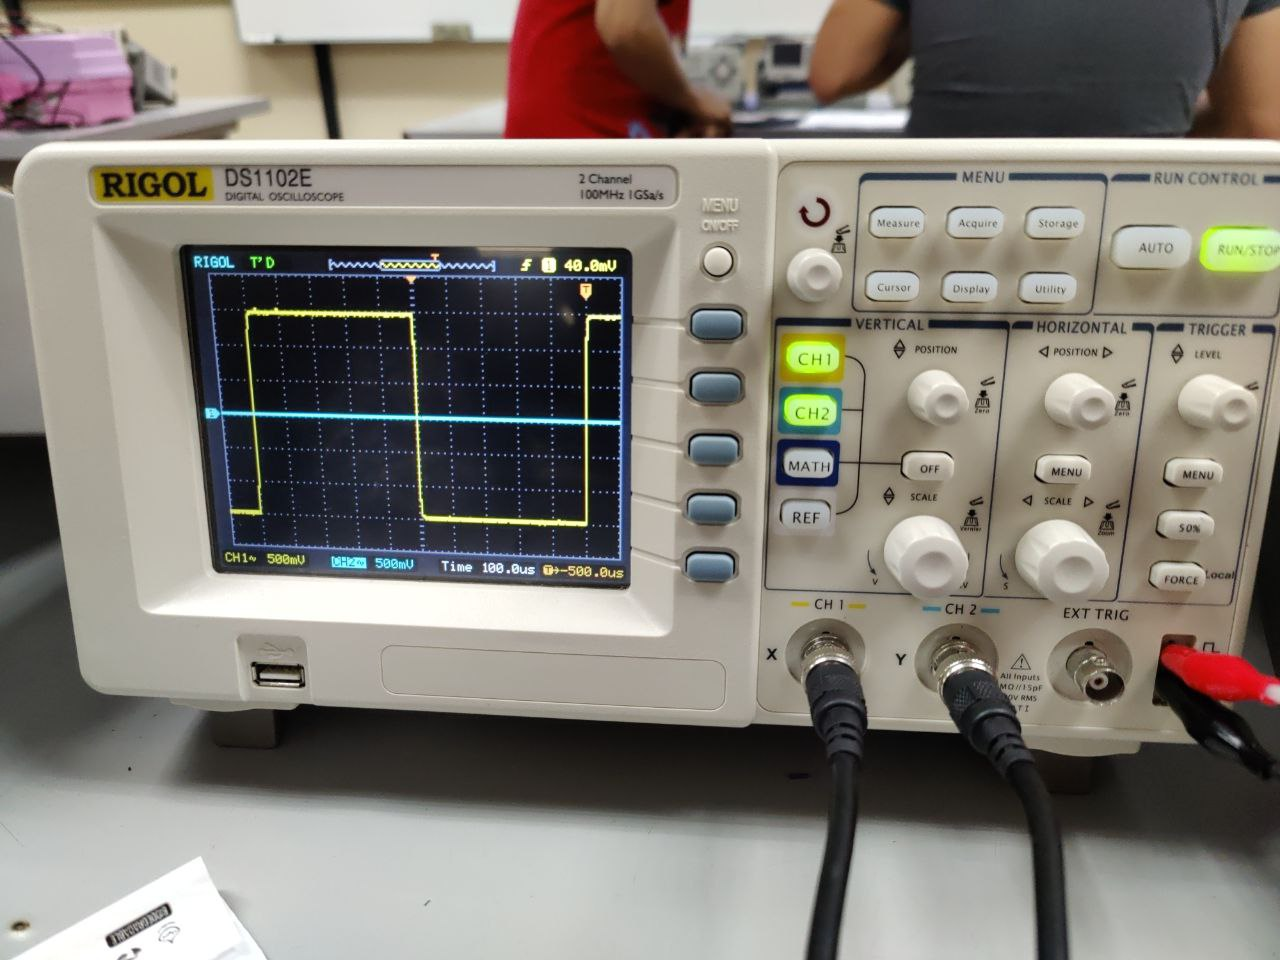
\includegraphics[width=.7\textwidth]{fig2}
	\label{fig5}
	 \caption{Simulación del circuito en serie-paralelo de la Figura 2}
\end{figure}

\end{document}